% Map of each island
\begin{figure}[H]
\centering
	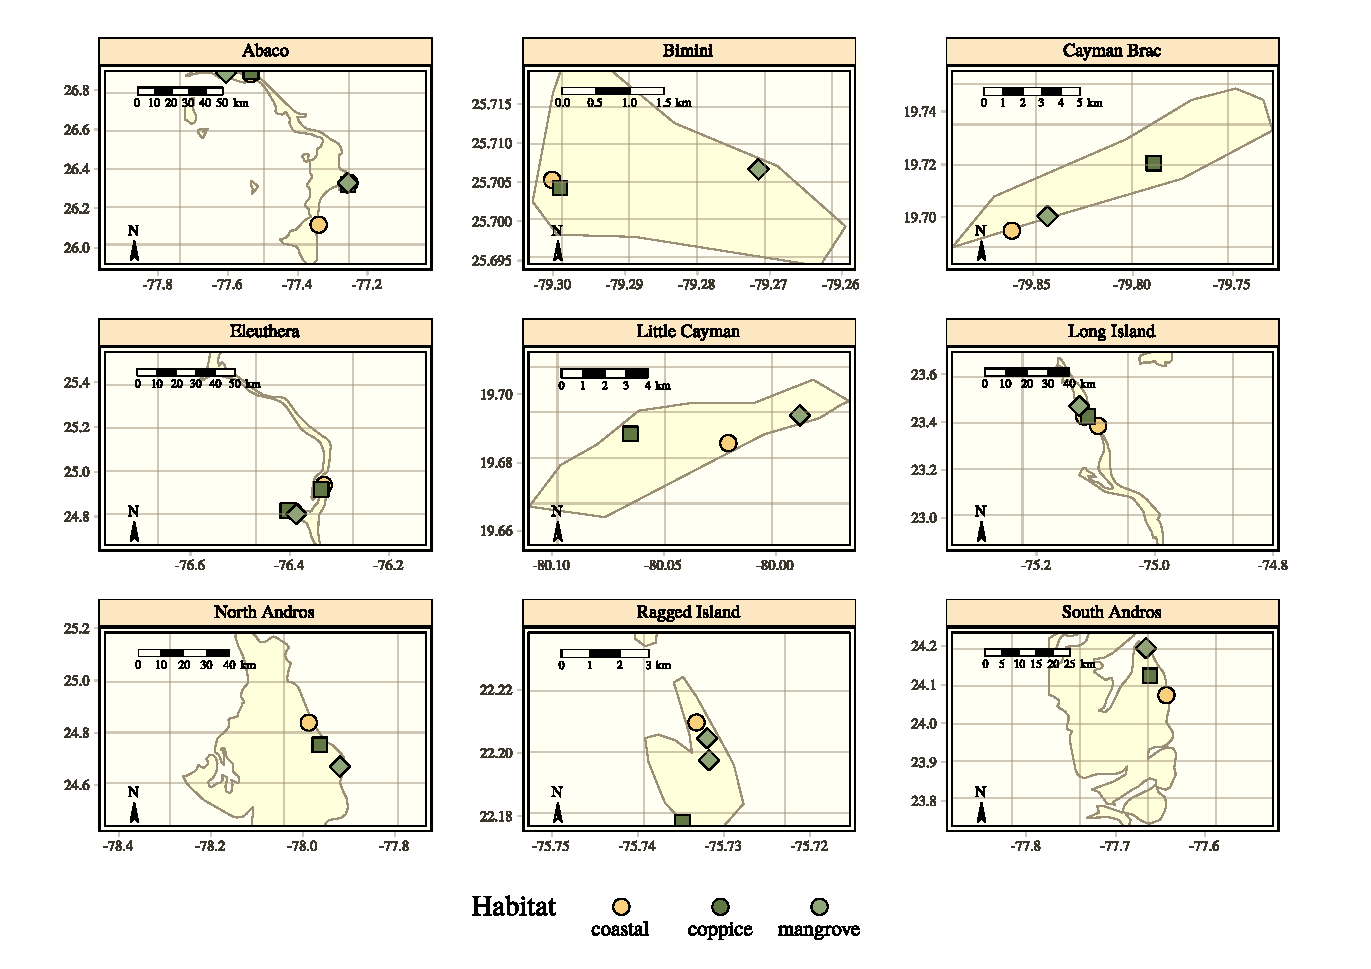
\includegraphics[width=\textwidth]{../maps/detailed_map.pdf}
	\caption{Map of the sampling sites and corresponding habitats across nine islands of the West Indies.}
	\label{supfig:map}
\end{figure}

\begin{figure}[H]
	\centering
	\includegraphics[width=0.8\textwidth]{"../analyses/03-PCA/figure_brightness"}
	\caption{Correlation between dewlap brightness (as measured by the mean reflectance from 300 to 700nm in wavelength) and PC1 score for each island. Pearson's squared correlation coefficients are reported. *, P < 0.05.}	
	\label{supfig:brightness}
\end{figure}

\begin{figure}[H]
	\centering
	\includegraphics[width=0.5\textwidth]{"../analyses/03-PCA/figure_brightness_pooled"}
	\caption{Correlation between dewlap brightness (as measured by the mean reflectance from 300 to 700nm in wavelength) and PC1 score across the whole archipelago. Pearson's squared correlation coefficient is reported. *, P < 0.05.}
	\label{supfig:brightness_pooled}
\end{figure}

\begin{figure}[H]
	\centering
	\includegraphics[width = \textwidth]{"../analyses/06-pooled/figure_pooled"}
	\caption{(A) Principal component scores and 5\% confidence ellipses across habitats for the whole archipelago. The principal component analysis was performed on reflectance data from all islands pooled together. (B) PCA rotation matrix showing the loadings of each wavelength from 300 to 700nm onto the principal components.}
	\label{supfig:pooled}
\end{figure}

% Reflectance curves
\begin{figure}[H]
	\centering
	\includegraphics[width=0.8\textwidth]{"../analyses/02-reflectance/figure_reflectance"}
	\caption{5-95th percentile range of lizard dewlap reflectance values (in \% of incoming light) across wavelengths for each island and each habitat.}
	\label{supfig:reflectance}
\end{figure}

\begin{figure}[H]
	\centering
	\includegraphics[width=0.8\textwidth]{"../analyses/04-machine learning/plots/classif_svm_pca_pooled"}
	\caption{Archipelago-wide SVM classification accuracy based on principal component data. Machines were trained on individual dewlaps regardless of island identity. The histogram shows the accuracy distribution over 100 replicates for each five cross-validation bins. The legend is the same as in Figure \ref{fig:classif-svm-pca}.}
	\label{supfig:classif-svm-pca-pooled}
\end{figure}

\begin{figure}[H]
	\centering
	\includegraphics[width=0.8\textwidth]{"../analyses/04-machine learning/plots/classif_svm_refl_pooled"}
	\caption{Archipelago-wide SVM classification accuracy based on reflectance data at 50nm-intervals in wavelength (see Methods). Machines were trained on individual dewlaps regardless of island identity. The histogram shows the accuracy distribution over 100 replicates for each five cross-validation bins. The legend is the same as in Figure \ref{fig:classif-svm-pca}.}
	\label{supfig:classif-svm-refl-pooled}
\end{figure}

\begin{figure}[H]
	\centering
	\includegraphics[width=0.4\textwidth]{"../analyses/04-machine learning/plots/importance_svm_pca_pooled"}
	\caption{Sensitivity analyses of the different input variables in the archipelago-wide SVM classification on principal component data (Figure \ref{supfig:classif-svm-pca-pooled}), with relative importance computed for every machine.}
	\label{supfig:importance-svm-pca-pooled}
\end{figure}

\begin{figure}[H]
	\centering
	\includegraphics[width=0.6\textwidth]{"../analyses/04-machine learning/plots/importance_svm_refl_pooled"}
	\caption{Sensitivity analyses of the different input variables in the archipelago-wide SVM classification on reflectance data at 50nm-intervals in wavelength (Figure \ref{supfig:classif-svm-refl-pooled}), with relative importance computed for every machine.}
	\label{supfig:importance-svm-refl-pooled}
\end{figure}

\begin{figure}[H]
	\centering
	\includegraphics[width=0.8\textwidth]{"../analyses/04-machine learning/plots/classif_lda_pca_pooled"}
	\caption{Archipelago-wide LDA classification accuracy based on principal component data. Machines were trained on individual dewlaps regardless of island identity. The histogram shows the accuracy distribution over 100 replicates for each five cross-validation bins. The legend is the same as in Figure \ref{fig:classif-svm-pca}.}
	\label{supfig:classif-lda-pca-pooled}
\end{figure}

\begin{figure}[H]
	\centering
	\includegraphics[width=0.8\textwidth]{"../analyses/04-machine learning/plots/classif_lda_refl_pooled"}
	\caption{Archipelago-wide LDA classification accuracy based on reflectance data at 50nm-intervals in wavelength (see Methods). Machines were trained on individual dewlaps regardless of island identity. The histogram shows the accuracy distribution over 100 replicates for each five cross-validation bins. The legend is the same as in Figure \ref{fig:classif-svm-pca}.}
	\label{supfig:classif-lda-refl-pooled}
\end{figure}

\begin{figure}[H]
	\centering
	\includegraphics[width=\textwidth]{"../analyses/04-machine learning/plots/classif_lda_pca"}
	\caption{LDA classification accuracy across islands based on principal component data. Histograms show accuracy distributions over 100 replicates for each five cross-validation bins per island. The legend is the same as in Figure \ref{fig:classif-svm-pca}.}
	\label{supfig:classif-lda-pca}
\end{figure}

\begin{figure}[H]
	\centering
	\includegraphics[width=\textwidth]{"../analyses/04-machine learning/plots/classif_svm_refl"}
	\caption{SVM classification accuracy across islands based on reflectance data at 50nm-intervals in wavelength (see Methods). Histograms show accuracy distributions over 100 replicates for each five cross-validation bins per island. The legend is the same as in Figure \ref{fig:classif-svm-pca}.}
	\label{supfig:classif-svm-refl}
\end{figure}

\begin{figure}[H]
	\centering
	\includegraphics[width=\textwidth]{"../analyses/04-machine learning/plots/classif_lda_refl"}
	\caption{LDA classification accuracy across islands based on reflectance data at 50nm-intervals in wavelength (see Methods). Histograms show accuracy distributions over 100 replicates for each five cross-validation bins per island. The legend is the same as in Figure \ref{fig:classif-svm-pca}.}
	\label{supfig:classif-lda-refl}
\end{figure}

\begin{figure}[H]
	\centering
	\includegraphics[width=0.8\textwidth]{"../analyses/04-machine learning/plots/importance_svm_pca"}
	\caption{Sensitivity analyses of the different input variables in the within-island SVM classification on principal component data (Figure \ref{supfig:classif-svm-pca}), with relative importance computed for every machine.}
	\label{supfig:importance-svm-pca}
\end{figure}

\begin{figure}[H]
	\centering
	\includegraphics[width=0.8\textwidth]{"../analyses/04-machine learning/plots/importance_lda_pca"}
	\caption{Sensitivity analyses of the different input variables in the within-island LDA classification on principal component data (Figure \ref{supfig:classif-lda-pca}), with relative importance computed for every machine.}
	\label{supfig:importance-lda-pca}
\end{figure}

\begin{figure}[H]
	\centering
	\includegraphics[width=0.8\textwidth]{"../analyses/04-machine learning/plots/importance_svm_pca"}
	\caption{Sensitivity analyses of the different input variables in the archipelago-wide SVM classification on reflectance at 50nm-intervals in wavelength (Figure \ref{supfig:classif-svm-refl}), with relative importance computed for every machine.}
	\label{supfig:importance-svm-refl}
\end{figure}

\begin{figure}[H]
	\centering
	\includegraphics[width=0.8\textwidth]{"../analyses/04-machine learning/plots/importance_lda_pca"}
	\caption{Sensitivity analyses of the different input variables in the archipelago-wide LDA classification on reflectance at 50nm-intervals in wavelength (Figure \ref{supfig:classif-lda-refl}), with relative importance computed for every machine.}
	\label{supfig:importance-lda-refl}
\end{figure}

\begin{figure}[H]
	\centering
	\includegraphics[width=\textwidth]{"../analyses/10-distances/figure_distances2"}
	\caption{Spatial scale of between-habitat differences in dewlap coloration. For each variable and each pair of habitats where significant differences were detected (Figure \ref{fig:anova}), we performed multiple post hoc pairwise comparisons between the sites involved (Figure \ref{supfig:map}, Table \ref{suptab:sites}), using nonparametric Wilcoxon-Mann-Whitney tests. Here we report, for each pair of habitats, the distances between sites that significantly differed in dewlap coloration at an error rate of 0.05 (P-values corrected with the Benjamini-Hochberg procedure for multiple testing).}
	\label{supfig:distances}
\end{figure}

\begin{figure}[H]
	\centering
	\includegraphics[width=0.7\textwidth]{"../analyses/09-parallelism/figure_contrasts"}
	\caption{Test of parallel divergence between islands. Differences in habitat-means, or contrasts, are shown for two pairs of habitats for each principal component on each island, rescaled so the standard deviation of the means along each principal component is one. The contrasts represent the patterns of between-habtiat variation on each island, for a given principal component. The absence of clustering of islands by variable indicates that islands differ in their between-habitat divergence patterns. This is confirmed by a non-significant MANOVA test of the between versus within-variable variance in contrasts.}
	\label{supfig:contrasts}
\end{figure}